\documentclass[11pt,aspectratio=169]{beamer}

\usepackage{booktabs}
\usepackage{array}
\usepackage{tikz}
\usepackage{pgfplots}
\usepackage{xcolor}
\usepackage{amsmath}
\usepackage{mathtools}
\usetikzlibrary{positioning,calc,arrows.meta}
\pgfplotsset{compat=1.18}

\usetheme[titleformat=smallcaps,progressbar=frametitle]{metropolis}
\definecolor{UTburnt}{HTML}{BF5700}
\definecolor{LBJnavy}{HTML}{172A46}
\definecolor{softgray}{HTML}{F2F3F5}
\definecolor{midgray}{HTML}{6B7280}
\setbeamercolor{alerted text}{fg=UTburnt}
\setbeamercolor{frametitle}{bg=LBJnavy,fg=white}
\setbeamercolor{progress bar}{fg=UTburnt,bg=gray!25}
\setbeamercolor{block title}{bg=LBJnavy!10,fg=LBJnavy}
\setbeamercolor{block body}{bg=softgray}
\setbeamertemplate{navigation symbols}{}
\setbeamertemplate{itemize item}{\color{UTburnt}$\blacktriangleright$}
\setbeamertemplate{itemize subitem}{\color{UTburnt}$\bullet$}

\author{Sergio I. Garc\'ia-R\'ios}
\title{Describing Data and Distributions}
\subtitle{Center, Spread, and the Mathematics of Variation}
\institute{PA 311N: Data Analysis for Public Policy\\LBJ School of Public Affairs}
\date{September 14, 2026}

\newcommand{\yourturn}[1]{%
\begin{center}
\begin{minipage}{0.90\textwidth}
\begin{alertblock}{Your Turn}
#1
\end{alertblock}
\end{minipage}
\end{center}}

\newcommand{\ourturn}[1]{%
\begin{center}
\begin{minipage}{0.90\textwidth}
\begin{block}{Our Turn}
#1
\end{block}
\end{minipage}
\end{center}}

\begin{document}
\maketitle

% 2
\begin{frame}{Today we put numbers on what we see}
Last time, we used visualizations to identify patterns in data.

\vspace{0.6em}
Today we ask:
\begin{itemize}
  \item Where is the \alert{center} of a distribution?
  \item How much \alert{variation} is there?
  \item How do extreme observations affect our summaries?
  \item How can we translate a graph into a defensible numerical description?
\end{itemize}

\vfill
\begin{center}
\Large Visualization $\longrightarrow$ Calculation $\longrightarrow$ Interpretation
\end{center}
\end{frame}

% 3
\begin{frame}{A numerical distribution: four things to describe}
\begin{columns}[T,onlytextwidth]
\column{0.48\textwidth}
\begin{block}{1. Shape}
Symmetric? Skewed? One peak or several?
\end{block}
\begin{block}{2. Center}
What value represents a typical observation?
\end{block}
\column{0.48\textwidth}
\begin{block}{3. Spread}
How much do observations vary?
\end{block}
\begin{block}{4. Unusual observations}
Are there values that stand apart from the rest?
\end{block}
\end{columns}

\vfill
\alert{This is the same backbone we will use whenever we describe a quantitative variable.}
\end{frame}

% 4
\begin{frame}[standout]
\Large Start with the picture.\\[0.5em]
\normalsize Then decide which numbers make sense.
\end{frame}

% 5
\begin{frame}{Shape: symmetry, skewness, and modality}
\centering
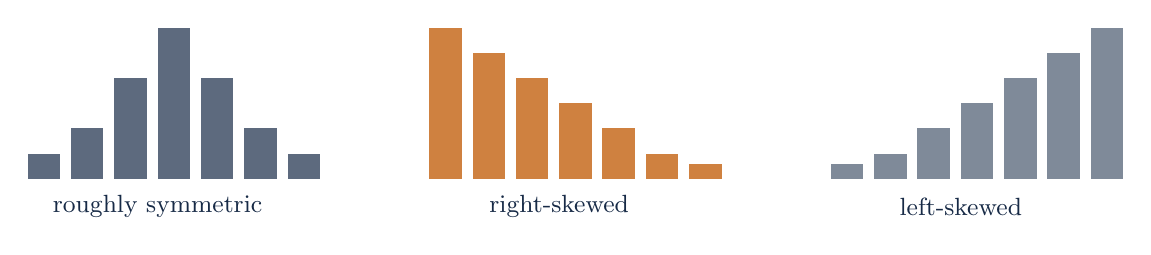
\begin{tikzpicture}[x=0.55cm,y=0.32cm]
% symmetric
\foreach \x/\h in {0/1,1/2,2/4,3/6,4/4,5/2,6/1}{\fill[LBJnavy!70] (\x,0) rectangle +(0.75,\h);}
\node[font=\small,LBJnavy] at (3,-1.1) {roughly symmetric};
% right skew
\begin{scope}[xshift=5.1cm]
\foreach \x/\h in {0/6,1/5,2/4,3/3,4/2,5/1,6/0.6}{\fill[UTburnt!75] (\x,0) rectangle +(0.75,\h);}
\node[font=\small,LBJnavy] at (3,-1.1) {right-skewed};
\end{scope}
% left skew
\begin{scope}[xshift=10.2cm]
\foreach \x/\h in {0/0.6,1/1,2/2,3/3,4/4,5/5,6/6}{\fill[LBJnavy!55] (\x,0) rectangle +(0.75,\h);}
\node[font=\small,LBJnavy] at (3,-1.1) {left-skewed};
\end{scope}
\end{tikzpicture}

\vspace{1.4em}
\begin{itemize}
  \item \alert{Skew} is named for the direction of the long tail.
  \item \alert{Modality} describes prominent peaks: unimodal, bimodal, and so on.
\end{itemize}
\end{frame}

% 6
\begin{frame}{Your turn: predict the shape before seeing data}
\yourturn{What shape would you expect for each variable? Explain why.
\begin{enumerate}
  \item Household income in a large U.S. city
  \item Scores on an easy exam
  \item Adult height within a single sex category
  \item Number of emergency-room visits in a year
\end{enumerate}}

\vfill
\small
Think about natural lower or upper bounds and the possibility of a few extreme values.
\end{frame}

% 7
\begin{frame}[standout]
\Large What is a ``typical'' observation?
\end{frame}

% 8
\begin{frame}{The sample mean}
For a sample of $n$ observations, the mean is

\[
\boxed{\bar{x}=\frac{1}{n}\sum_{i=1}^{n} x_i}
\]

\vspace{0.6em}
In words:
\[
\text{mean}=\frac{\text{sum of all observed values}}{\text{number of observations}}
\]

\vfill
\begin{block}{Notation matters}
$\bar{x}$ = sample mean \qquad $\mu$ = population mean
\end{block}
\end{frame}

% 9
\begin{frame}{Our turn: calculate a mean}
\ourturn{Suppose five neighborhoods have an illustrative policy score of
\[
2,\;4,\;5,\;7,\;12.
\]
What is the sample mean?}

\[
\bar{x}=\frac{2+4+5+7+12}{5}=\frac{30}{5}=\boxed{6}
\]

\vfill
\alert{The mean uses every observation in the dataset.}
\end{frame}

% 10
\begin{frame}{The mean is a balance point}
Using the same data, $\bar{x}=6$.

\begin{center}
\renewcommand{\arraystretch}{1.25}
\begin{tabular}{r|rrrrr|r}
$x_i$ & 2 & 4 & 5 & 7 & 12 & \\
\midrule
$x_i-\bar{x}$ & $-4$ & $-2$ & $-1$ & $1$ & $6$ & $0$ \\
\end{tabular}
\end{center}

\vspace{0.8em}
\[
\sum_{i=1}^{n}(x_i-\bar{x})=0
\]

\vfill
\begin{alertblock}{Important}
Positive and negative deviations from the mean exactly cancel. This will matter when we measure spread.
\end{alertblock}
\end{frame}

% 11
\begin{frame}{The median}
The \alert{median} is the middle value after sorting observations from smallest to largest.

\vspace{0.5em}
\begin{columns}[T,onlytextwidth]
\column{0.46\textwidth}
\begin{block}{Odd number of observations}
\[
2,\;4,\;\boxed{5},\;7,\;12
\]
Median $=5$.
\end{block}
\column{0.46\textwidth}
\begin{block}{Even number of observations}
\[
2,\;4,\;\boxed{5,\;7},\;12,\;14
\]
Median $=(5+7)/2=6$.
\end{block}
\end{columns}

\vfill
\alert{The median depends on order, not the exact distance between values.}
\end{frame}

% 12
\begin{frame}{Mean vs. median: add one extreme value}
\yourturn{How do the mean and median change?}

\begin{columns}[T,onlytextwidth]
\column{0.47\textwidth}
\begin{block}{Dataset A}
\[
30,\;50,\;70,\;90
\]
\[
\bar{x}=60,\qquad \text{median}=60
\]
\end{block}
\column{0.47\textwidth}
\begin{block}{Dataset B}
\[
30,\;50,\;70,\;1000
\]
\[
\bar{x}=287.5,\qquad \text{median}=60
\]
\end{block}
\end{columns}

\vfill
\alert{The mean moves dramatically. The median does not.}
\end{frame}

% 13
\begin{frame}{Why policy analysts often care about the median}
Imagine five illustrative home values, in thousands of dollars:
\[
250,\;275,\;300,\;325,\;1200
\]

\begin{columns}[T,onlytextwidth]
\column{0.45\textwidth}
\begin{block}{Mean}
\[
\bar{x}=470
\]
$\$470{,}000$
\end{block}
\column{0.45\textwidth}
\begin{block}{Median}
\[
\tilde{x}=300
\]
$\$300{,}000$
\end{block}
\end{columns}

\vfill
\yourturn{Which number better describes a ``typical'' home in this tiny example? What information does the other number still convey?}
\end{frame}

% 14
\begin{frame}[standout]
\Large Center is not enough.
\end{frame}

% 15
\begin{frame}{Same center, very different spread}
\begin{columns}[T,onlytextwidth]
\column{0.47\textwidth}
\begin{block}{Dataset A}
\[
4,\;5,\;6,\;7,\;8
\]
Mean $=6$
\end{block}
\column{0.47\textwidth}
\begin{block}{Dataset B}
\[
0,\;3,\;6,\;9,\;12
\]
Mean $=6$
\end{block}
\end{columns}

\vspace{0.8em}
\begin{center}
\Large Same center. \alert{Different variation.}
\end{center}

\vfill
A useful description of a quantitative variable usually needs both center \emph{and} spread.
\end{frame}

% 16
\begin{frame}{The range}
The simplest measure of spread is
\[
\boxed{\text{Range}=\max(x)-\min(x)}
\]

For
\[
2,\;4,\;5,\;7,\;12,
\]

\[
\text{Range}=12-2=10.
\]

\vfill
\begin{alertblock}{Limitation}
The range depends only on the two most extreme observations.
\end{alertblock}
\end{frame}

% 17
\begin{frame}{Quartiles and the interquartile range}
Quartiles divide ordered data into four parts.

\begin{center}
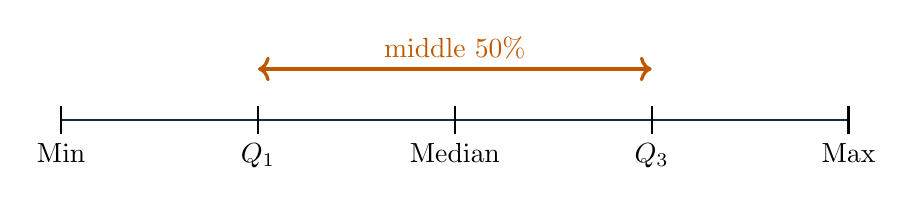
\begin{tikzpicture}[x=1.25cm]
\draw[thick,LBJnavy] (0,0)--(8,0);
\foreach \x/\lab in {0/Min,2/$Q_1$,4/Median,6/$Q_3$,8/Max}{
  \draw[thick] (\x,-0.18)--(\x,0.18);
  \node[below=5pt] at (\x,0) {\lab};
}
\draw[very thick,UTburnt,<->] (2,0.65)--(6,0.65);
\node[above,UTburnt] at (4,0.65) {middle 50\%};
\end{tikzpicture}
\end{center}

\[
\boxed{IQR=Q_3-Q_1}
\]

\vfill
\alert{The IQR measures the spread of the middle 50\% of observations.}
\end{frame}

% 18
\begin{frame}{Our turn: quartiles and IQR}
Use the \textbf{median-of-halves} convention for today.

\[
2,\;4,\;5,\;7,\;8,\;10,\;12,\;14
\]

\begin{columns}[T,onlytextwidth]
\column{0.47\textwidth}
\[
\text{Median}=\frac{7+8}{2}=7.5
\]
\[
Q_1=\frac{4+5}{2}=4.5
\]
\column{0.47\textwidth}
\[
Q_3=\frac{10+12}{2}=11
\]
\[
IQR=11-4.5=\boxed{6.5}
\]
\end{columns}

\vfill
\footnotesize Different software can use slightly different quartile conventions for some datasets. The underlying idea is the same.
\end{frame}

% 19
\begin{frame}{A boxplot compresses the distribution}
\centering
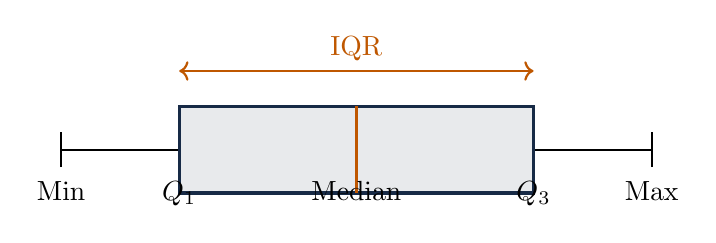
\begin{tikzpicture}[x=0.75cm,y=1cm]
\draw[thick] (0,0)--(2,0);
\draw[thick] (8,0)--(10,0);
\draw[thick] (0,-0.22)--(0,0.22);
\draw[thick] (10,-0.22)--(10,0.22);
\draw[very thick,LBJnavy,fill=LBJnavy!10] (2,-0.55) rectangle (8,0.55);
\draw[very thick,UTburnt] (5,-0.55)--(5,0.55);
\node[below=8pt] at (0,0) {Min};
\node[below=8pt] at (2,0) {$Q_1$};
\node[below=8pt] at (5,0) {Median};
\node[below=8pt] at (8,0) {$Q_3$};
\node[below=8pt] at (10,0) {Max};
\draw[UTburnt,<->,thick] (2,1.0)--(8,1.0);
\node[above,UTburnt] at (5,1.0) {IQR};
\end{tikzpicture}

\vspace{1.0em}
A boxplot makes it easy to compare \alert{center}, \alert{spread}, \alert{skew}, and possible \alert{outliers}.
\end{frame}

% 20
\begin{frame}{The 1.5 $\times$ IQR rule for suspected outliers}
A common rule flags observations outside these fences:

\[
\boxed{\text{Lower fence}=Q_1-1.5(IQR)}
\]
\[
\boxed{\text{Upper fence}=Q_3+1.5(IQR)}
\]

\vspace{0.7em}
An observation beyond a fence is a \alert{suspected outlier}.

\vfill
\begin{alertblock}{Do not automatically delete it.}
An unusual value may be an error, but it may also be the most substantively important case in the dataset.
\end{alertblock}
\end{frame}

% 21
\begin{frame}{Our turn: is 30 an outlier?}
Consider
\[
2,\;4,\;5,\;7,\;8,\;10,\;12,\;30.
\]
Using the median-of-halves convention:
\[
Q_1=4.5,\qquad Q_3=11,\qquad IQR=6.5.
\]

\[
\text{Lower fence}=4.5-1.5(6.5)=-5.25
\]
\[
\text{Upper fence}=11+1.5(6.5)=20.75
\]

\begin{center}
\Large $30>20.75$ \qquad $\Rightarrow$ \qquad \alert{30 is a suspected outlier.}
\end{center}
\end{frame}

% 22
\begin{frame}[standout]
\Large How far are observations from the mean?
\end{frame}

% 23
\begin{frame}{Why not just average the deviations?}
For
\[
2,\;4,\;5,\;7,\;12, \qquad \bar{x}=6,
\]
we have:

\begin{center}
\renewcommand{\arraystretch}{1.25}
\begin{tabular}{r|rrrrr}
$x_i$ & 2 & 4 & 5 & 7 & 12 \\
\midrule
$x_i-\bar{x}$ & $-4$ & $-2$ & $-1$ & $1$ & $6$ \\
\end{tabular}
\end{center}

\[
-4-2-1+1+6=0.
\]

\vfill
\alert{The deviations always sum to zero, so their ordinary average cannot measure spread.}
\end{frame}

% 24
\begin{frame}{The solution: square the deviations}
Squaring does two useful things:
\begin{enumerate}
  \item removes negative signs;
  \item gives larger deviations more weight.
\end{enumerate}

\vspace{0.7em}
\begin{center}
\renewcommand{\arraystretch}{1.25}
\begin{tabular}{r|rrrrr}
$x_i-\bar{x}$ & $-4$ & $-2$ & $-1$ & $1$ & $6$ \\
\midrule
$(x_i-\bar{x})^2$ & 16 & 4 & 1 & 1 & 36 \\
\end{tabular}
\end{center}

\[
\sum (x_i-\bar{x})^2=58.
\]
\end{frame}

% 25
\begin{frame}{Sample variance}
The sample variance is the average squared distance from the mean, with an adjustment for estimating the mean from the same sample:

\[
\boxed{s^2=\frac{\sum_{i=1}^{n}(x_i-\bar{x})^2}{n-1}}
\]

For our five observations:
\[
s^2=\frac{58}{5-1}=\frac{58}{4}=\boxed{14.5}.
\]

\vfill
\begin{block}{Units}
If $x$ is measured in points, variance is measured in \emph{points squared}.
\end{block}
\end{frame}

% 26
\begin{frame}{Standard deviation brings us back to the original units}
Take the square root of the variance:

\[
\boxed{s=\sqrt{s^2}=\sqrt{\frac{\sum_{i=1}^{n}(x_i-\bar{x})^2}{n-1}}}
\]

For our example:
\[
s=\sqrt{14.5}\approx\boxed{3.81}.
\]

\vfill
\begin{alertblock}{Interpretation}
The standard deviation summarizes the typical scale of distance between observations and the mean. Smaller $s$ means values are more tightly clustered; larger $s$ means more variation.
\end{alertblock}
\end{frame}

% 27
\begin{frame}{Put the entire calculation together}
For $2,4,5,7,12$, $\bar{x}=6$.

\begin{center}
\renewcommand{\arraystretch}{1.25}
\begin{tabular}{rcc}
\toprule
$x_i$ & $x_i-\bar{x}$ & $(x_i-\bar{x})^2$ \\
\midrule
2 & $-4$ & 16 \\
4 & $-2$ & 4 \\
5 & $-1$ & 1 \\
7 & $1$ & 1 \\
12 & $6$ & 36 \\
\midrule
 & Sum $=0$ & Sum $=58$ \\
\bottomrule
\end{tabular}
\end{center}

\[
s^2=58/4=14.5,\qquad s=\sqrt{14.5}=3.81.
\]
\end{frame}

% 28
\begin{frame}{Same mean, different standard deviation}
\begin{columns}[T,onlytextwidth]
\column{0.46\textwidth}
\begin{block}{Dataset A}
\[
4,5,6,7,8
\]
\[
\bar{x}=6,\qquad s\approx1.58
\]
\end{block}
\column{0.46\textwidth}
\begin{block}{Dataset B}
\[
0,3,6,9,12
\]
\[
\bar{x}=6,\qquad s\approx4.74
\]
\end{block}
\end{columns}

\vfill
\yourturn{What does the larger standard deviation tell us substantively about Dataset B?}
\end{frame}

% 29
\begin{frame}{Why do we divide by $n-1$?}
When we calculate $s^2$, we already used the sample to estimate $\bar{x}$.

\vspace{0.6em}
Once $n-1$ deviations are known, the final deviation is forced because
\[
\sum (x_i-\bar{x})=0.
\]

That leaves \alert{$n-1$ degrees of freedom}.

\vfill
\begin{block}{For now}
You should understand the intuition and recognize the formula. We will return to degrees of freedom when we study statistical inference.
\end{block}
\end{frame}

% 30
\begin{frame}{Robust and non-robust statistics}
\begin{center}
\renewcommand{\arraystretch}{1.4}
\begin{tabular}{lll}
\toprule
 & \textbf{Center} & \textbf{Spread} \\
\midrule
Sensitive to extremes & Mean & Standard deviation \\
More robust & Median & IQR \\
\bottomrule
\end{tabular}
\end{center}

\vspace{0.8em}
\begin{itemize}
  \item Roughly symmetric distribution, no major outliers: \alert{mean + SD}
  \item Strongly skewed distribution or important outliers: \alert{median + IQR}
\end{itemize}

\vfill
\begin{center}
\Large Look at the distribution \emph{before} choosing the summary.
\end{center}
\end{frame}

% 31
\begin{frame}{Your turn: what would you report?}
\yourturn{Choose a center and spread for each case, and explain your choice.
\begin{enumerate}
  \item Household income with a long right tail
  \item Adult heights with an approximately symmetric distribution
  \item Emergency-room wait times with several extremely long waits
  \item Scores on an exam with no strong skew or outliers
\end{enumerate}}

\vfill
\small
Do not choose based on habit. Choose based on what the distribution looks like.
\end{frame}

% 32
\begin{frame}{From hand calculation to R}
You should understand what the statistics mean before asking software to compute them.

\vspace{0.5em}
\begin{block}{Common R functions}
\ttfamily
mean(x)\\
median(x)\\
range(x)\\
IQR(x)\\
var(x)\\
sd(x)\\
summary(x)
\end{block}

\vfill
\alert{R does the arithmetic. You still decide what to calculate and how to interpret it.}
\end{frame}

% 33
\begin{frame}{A complete descriptive statement}
Suppose a distribution is right-skewed with a median of 18 minutes and an IQR of 11 minutes.

\vspace{0.8em}
A strong description might say:

\begin{quote}
``Wait times are right-skewed. The median wait is 18 minutes, and the middle 50\% of observations span 11 minutes. A small number of substantially longer waits produce the right tail.''
\end{quote}

\vfill
\begin{alertblock}{Notice}
Shape + center + spread + unusual observations = a substantive description.
\end{alertblock}
\end{frame}

% 34
\begin{frame}{Exit check}
For the data
\[
3,\;4,\;5,\;6,\;7,\;8,\;23,
\]
work with a partner and answer:

\begin{enumerate}
  \item What are the mean and median?
  \item Which is more representative of a typical value?
  \item What is the range?
  \item Would you prefer mean + SD or median + IQR? Why?
  \item What would you inspect before calling 23 an error?
\end{enumerate}
\end{frame}

% 35
\begin{frame}{What I want you to leave with}
\begin{enumerate}
  \item \textbf{Start with the distribution.} Describe shape and unusual observations.
  \item \textbf{Center needs context.} Mean and median answer related but different questions.
  \item \textbf{Spread matters.} Two datasets can have the same center and very different variation.
  \item \textbf{Know the mathematics.} Variance and standard deviation are built from deviations from the mean.
  \item \textbf{Match the statistics to the data.} Mean + SD for roughly symmetric data; median + IQR for skewed data or outliers.
\end{enumerate}

\vfill
\begin{center}
\Large \alert{See it. Calculate it. Interpret it.}
\end{center}
\end{frame}

\end{document}
